\documentclass[12pt]{article}
\usepackage{xeCJK}
\usepackage{float}
\usepackage{indentfirst}
\usepackage{booktabs}
\usepackage{geometry}  
\usepackage{titlesec}   
\usepackage{array}
\usepackage{multirow}
\usepackage{listings}
\usepackage{titlesec} 
\usepackage{amsmath}
\usepackage{graphicx}
% \pagestyle{fancy} 
\geometry{left=2.5cm,right=3.5cm,top=2.5cm,bottom=2.5cm}

\setlength{\parindent}{2em}
\linespread{1.3}

\date{}
\begin{document}
\newpagestyle{main}{            
    \sethead{题解}{}{\sectiontitle}     %设置页眉
    \setfoot{}{第\thepage 页,共3页}{}      %设置页脚,可以在页脚添加 \thepage  显示页数
    \headrule                                      % 添加页眉的下划线
    \footrule                                       %添加页脚的下划线
}
\pagestyle{main}

\section{T1 废墟}

考虑将$1$到$n$从大到小插入这个排列,我们不妨设$k = m - n$,那么此时$1, 2, \cdots, k$可以与任何数相邻。记此时的方案数为$F(n, k)$,可以发现当$n = k$或$n = k + 1$时$F(n, k) = n!$。\par
对于剩余的情况,有$k\leq n - 2$。如果此时$n$在整个序列的最左边或者最右边,不妨假设在最左边,那么与它相邻的数一共有$k$种填法,剩下$n - 2$个数未选择。此时我们随便从这$n - 2$个数中拿出一个数出来填入第三个位置都是合法的。最大的数变为了$n - 1$,因此此时剩下的可以与任何数相邻的数的个数没有变化,方案数为$2kF(n - 2, k)$\par
如果$n$在序列的中间,那么它左右的邻居共有$k(k - 1)$种选法。此时我们将这三个位置缩在一起作为一个整体参与接下来的排列。同样,此时剩下了$n - 2$个数,最大的数减少了$1$,而这三个数缩在一起之后产生的新的元素可以与任何数相邻,剩下的可以与任何数相邻的数的个数没有变化,因此方案数为$k(k - 1)F(n - 2, k)$\par
综合以上两种情况,可以得到最终的转移:

$$\begin{aligned}
    F(n, k) &= 2kF(n - 2, k) + k(k - 1)F(n - 2, k) \\
    &= k(k + 1)F(n - 2, k) 
\end{aligned}$$

事实上,直接打表也可以很容易地得到这个转移。

\newpage

\section{T2 魔法}

树上的简单路径$(u, v)$只有两种:要么$(u, v)$中其中一个是祖先,要么它们跨过了它们的$\mathrm{lca}$。考虑对于这两种路径分别计数。\par
对于第一种路径,可以发现路径上的点数减去每个点在路径上的儿子数量恰好为$1$。假如我们现在要判断所有$\leq L$的点是否形成了一条简单路径,可以利用这个性质,统计有多少个点满足这个点的权值$\leq L$,且存在某个儿子的权值$\leq L$,我们将这种点称为$A$类点。记$c$为$A$类点的数量,那么当且仅当$L - c = 1$时这$L$个点才能构成这种路径。

对于第二种路径,沿用统计第一种路径的思路,相当于存在一个点,满足这个点$\leq L$,存在两个儿子$\leq L$,且这个点的父亲$>L$,我们将这种点称为$B$类点。此时若简单路径存在,则必须满足$L - c = 2$,且存在$B$类点。需要注意的是$B$类点同时也是一种特殊的$A$类点。

使用线段树维护每个$L$减去$c$之后的值,同时维护区间最小值以及最小值的出现次数,一开始线段树上位置$i$的值为$i$。对于一个非叶子节点$u$,假设它的权值为$p_u$,它的权值最小的儿子的权值为$q_u$,那么当$L\geq \max(p_u, q_u)$时,这个点将作为一个$A$类点出现;如果它的次小儿子的权值为$q'_u$,那么当$L\in[\max(p_u, q'_u), p_{fa_u}]$时,这个点将会作为一个$B$类点出现。

维护所有的$A$类点的同时,开一个全局set维护所有的$B$类点。查询的时候拿出权值最小的$B$类点,假设它的出现区间为$[l, r]$,那么就在线段树上将区间$[l, r]$全部$-1$,然后查询全局最小值的个数即可。

修改仅会影响到至多$4$个点:$u$,$v$,$u$的父亲以及$v$的父亲,对于这$4$个点重新统计即可,更多的细节可以参考标程。

\newpage

\section{T3 风暴}

我们新建第$0$行,然后假设$(0, 1)$与$(1, 1)$的连边必定不会断开,$(0, x)$与$(1, x)$的连边必定断开,接下来考虑轮廓线dp。考虑按列计算,计算到$(r, c)$时,我们存下$(r, c), (r - 1, c), \cdots, (0, c), (r + 1, c - 1), (r + 1, c - 1), \cdots, (n, c - 1)$的连通状态。

\begin{center}
    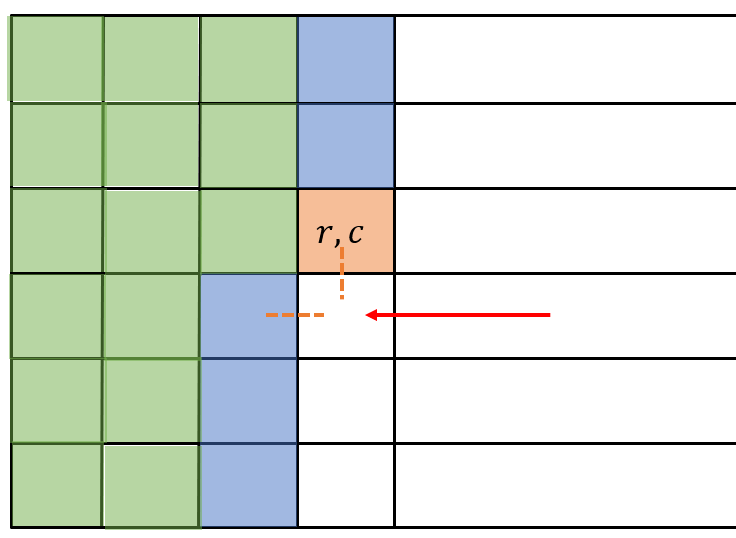
\includegraphics[scale = 0.5]{1.png}
\end{center}

在某个状态中,我们给每个格子分配一个数,如果两个格子的数相同则说明这两个格子处于同一个连通块。当$n = 8$时状态总数为$3432$。\par
从$(r, c)$转移到$(r + 1, c)$时,枚举图中两条边的连接状态,可以计算出接下来的状态。注意转移的时候需要保证当前维护的格子中,至少有一个格子与$(0, c)$连通。\par
当$m$比较小$(\leq 50)$的时候可以直接暴力转移,同时我们可以发现这样一个性质:设$m = k$时的答案为$ans_k$,那么当$k$很大时$\frac{ans_{k + 1}}{ans_k}$将趋近于一个定值,并且这个值收敛得很快。因此此时对于前$50$列我们暴力转移,然后直接$pow$算出最终的答案。

\end{document}